\documentclass[a4paper, 10pt, ]{article}

\usepackage[slovak]{babel}

\usepackage[utf8]{inputenc}
\usepackage[T1]{fontenc}

\usepackage[left=4cm,
			right=4cm,
			top=2.1cm,
			bottom=2.6cm,
			footskip=7.5mm,
			twoside,
			marginparwidth=3.5cm,
			%showframe,
			]{geometry}

\usepackage{graphicx}
\usepackage[dvipsnames]{xcolor}

% ------------------------------

\usepackage{lmodern}

\usepackage[tt={oldstyle=false,proportional=true,monowidth}]{cfr-lm}

% ------------------------------

\usepackage{amsmath}
\usepackage{amssymb}
\usepackage{amsthm}

\usepackage{booktabs}
\usepackage{multirow}
\usepackage{array}
\usepackage{dcolumn}

\usepackage{natbib}

\usepackage[singlelinecheck=true]{subfig}


% ------------------------------


\usepackage{sectsty}
\allsectionsfont{\sffamily}


\usepackage{titlesec}
\titleformat{\paragraph}[hang]{\sffamily  \bfseries}{}{0pt}{}
\titlespacing*{\paragraph}{0mm}{3mm}{1mm}


\usepackage{fancyhdr}
\fancypagestyle{plain}{%
\fancyhf{} % clear all header and footer fields
\fancyfoot[C]{\sffamily {\bfseries \thepage}\ | {\scriptsize\oznacenieCasti}}
\renewcommand{\headrulewidth}{0pt}
\renewcommand{\footrulewidth}{0pt}}
\pagestyle{plain}


% ------------------------------


\makeatletter

	\def\@seccntformat#1{\protect\makebox[0pt][r]{\csname the#1\endcsname\hspace{5mm}}}

	\def\cleardoublepage{\clearpage\if@twoside \ifodd\c@page\else
	\hbox{}
	\vspace*{\fill}
	\begin{center}
	\phantom{}
	\end{center}
	\vspace{\fill}
	\thispagestyle{empty}
	\newpage
	\if@twocolumn\hbox{}\newpage\fi\fi\fi}

	\newcommand\figcaption{\def\@captype{figure}\caption}
	\newcommand\tabcaption{\def\@captype{table}\caption}

\makeatother


% ------------------------------


\def\naT{\mathsf{T}}

\hyphenpenalty=6000
\tolerance=6000


% ------------------------------


\usepackage[pdfauthor={},
			pdftitle={},
			pdfsubject={},
			pdfkeywords={},
			% hidelinks,
			colorlinks=true,
			breaklinks,
			]{hyperref}






% ------------------------------

\usepackage{enumitem}





\usepackage[titles]{tocloft}

\setlength{\cftsecindent}{-12mm}
\setlength{\cftsecnumwidth}{12mm}
\renewcommand{\cftsecpresnum}{\hfill}
\renewcommand{\cftsecaftersnum}{\hspace{4mm}}

\setlength{\cftsubsecindent}{-12mm}
\setlength{\cftsubsecnumwidth}{16mm} % 12 + 4
\renewcommand{\cftsubsecpresnum}{\hfill}
\renewcommand{\cftsubsecaftersnum}{\hspace{8mm}} % 4 + 4 mm

\setlength{\cftsubsubsecindent}{-12mm}
\setlength{\cftsubsubsecnumwidth}{20mm} % 12 + 4 + 4
\renewcommand{\cftsubsubsecpresnum}{\hfill}
\renewcommand{\cftsubsubsecaftersnum}{\hspace{12mm}} % 4 + 4 + 4 mm

\renewcommand{\cftsecpagefont}{\lstyle \bfseries}
\renewcommand{\cftsubsecpagefont}{\lstyle}
\renewcommand{\cftsubsubsecpagefont}{\lstyle}



\setlength{\cftparaindent}{-16mm}
\setlength{\cftparanumwidth}{28mm} % 16 + 4 + 4 + 4
\renewcommand{\cftparapresnum}{\hfill}
\renewcommand{\cftparaaftersnum}{\hspace{16mm}} % 4 + 4 + 4 + 4 mm

% ------------------------------









\usepackage{listings}



\renewcommand{\lstlistingname}{Výpis kódu}
\renewcommand{\lstlistlistingname}{Výpisy kódu}




%New colors defined below
\definecolor{codegreen}{rgb}{0,0.6,0}
\definecolor{codegray}{rgb}{0.5,0.5,0.5}
\definecolor{codepurple}{rgb}{0.58,0,0.82}
\definecolor{backcolour}{rgb}{0.95,0.95,0.95}

%Code listing style named "mystyle"
\lstdefinestyle{mystyle}{
  backgroundcolor=\color{backcolour},
  commentstyle=\fontfamily{lmtt}\fontsize{8.5pt}{8.75pt}\selectfont\color{codegreen},
  keywordstyle=\fontfamily{lmtt}\fontsize{8.5pt}{8.75pt}\selectfont\bfseries\color{Blue},
  stringstyle=\fontfamily{lmtt}\fontsize{8.5pt}{8.75pt}\selectfont\color{codepurple},
  basicstyle=\fontfamily{lmtt}\fontsize{8.5pt}{8.75pt}\selectfont,
  breakatwhitespace=false,
  breaklines=true,
  captionpos=t,
  keepspaces=true,
  numbers=left,
  numbersep=4mm,
  numberstyle=\fontfamily{lmtt}\fontsize{8.5pt}{8.75pt}\selectfont\color{lightgray},
  showspaces=false,
  showstringspaces=false,
  showtabs=false,
  tabsize=2,
  % xleftmargin=10pt,
  framesep=10pt,
  language=Python,
  escapechar=|,
}




% ------------------------------



\graphicspath{{fig/}{../../extObr/}}


\def\oznacenieCasti{cvUdK06 - ZS2019}





\begin{document}

\lstset{style=mystyle}


\fontsize{12pt}{22pt}\selectfont

\centerline{\textsf{Úvod do kybernetiky} \hfill \textsf{\oznacenieCasti}}

\fontsize{18pt}{22pt}\selectfont





\begin{flushleft}
    \textbf{\textsf{Meranie prechodových charakteristík}}
\end{flushleft}





\normalsize

\bigskip

\tableofcontents

\bigskip

\vspace{18pt}





\section{Úvod}


Nasledujúci text má za cieľ inšpirovať čitateľa tak, aby získal lepšiu predstavu o tom ako zrealizovať zmysluplné meranie prechodových charakteristík. V tomto prípade totiž nie je úlohou len samotné meranie. Potrebný je tiež rozbor problému z hľadiska daného reálneho systému (ktorého vlastnosti skúmame). Preto je v prvom rade potrebné vysvetlenie pojmov používaných pri opise dynamického systému.


Pripomeňme, že v tomto bode máme dostupnú istú informáciu o predmetnom skúmanom systéme. Je ňou prevodová charakteristika - viď obr.~\ref{Prevodová charakteristika graf}.



\begin{figure}[t]
	\centering

    \makebox[\textwidth][c]{%
	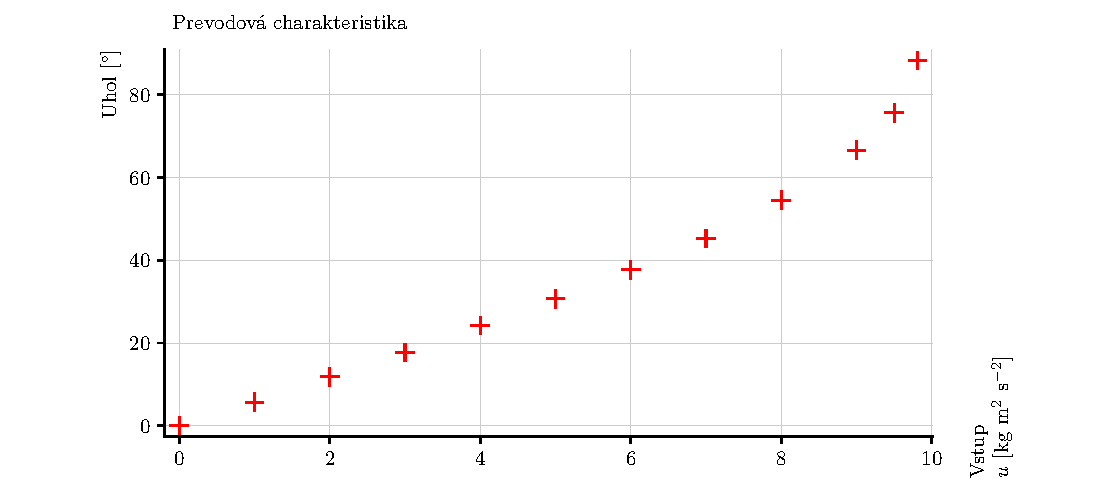
\includegraphics{../fig/cv07_fig_1.pdf}
	}

    \vspace{-4mm}

	\caption{}
	\label{Prevodová charakteristika graf}

\end{figure}


Samotná prevodová charakteristika vystihuje tzv. statické vlastnosti systému. Vlastnosti systému v ustálenom stave. Celkom konkrétne je možné z prevodovej charakteristiky získať statické zosilnenie systému.

Prevodová charakteristika na obr.~\ref{Prevodová charakteristika graf} ukazuje, že zosilnenie systému pri nižších hodnotách vstupného signálu je iné ako zosilnenie pri vyšších hodnotách vstupného signálu. Využime skutočnosť, že v tomto prípade máme dostupný model prevodovej charakteristiky (nie je nevyhnutné mať takýto model). Modelom je polynomiálna funkcia, konkrétne:
\begin{equation} \label{modelPolifitVysl}
    \hat y = 0,1111 u^3  -1,1150 u^2 + 8,9102 u  -1,1770
\end{equation}
Použime tento model pre vypočítanie výstupov (odhadov výstupov) systému v týchto hodnotách vstupného signálu:
\begin{lstlisting}[language=Matlab,]
u_ine = [0:0.1:9.81];
\end{lstlisting}
Získame nasledujúci obrázok (obr.~\ref{Prevodová charakteristika graf2}).



Obr.~\ref{Prevodová charakteristika graf2} len lepšie ilustruje rozdielne statické zosilnenie systému pri malých a pri veľkých hodnotách vstupného signálu. Aj v ďalších častiach tohto textu budeme využívať dostupnosť modelu. Tu naposledy spomenieme, že nie je nevyhnutné mať model pre uskutočnenie toho, o čom sa v nasledujúcom píše.








\begin{figure}[t]
	\centering

    \makebox[\textwidth][c]{%
	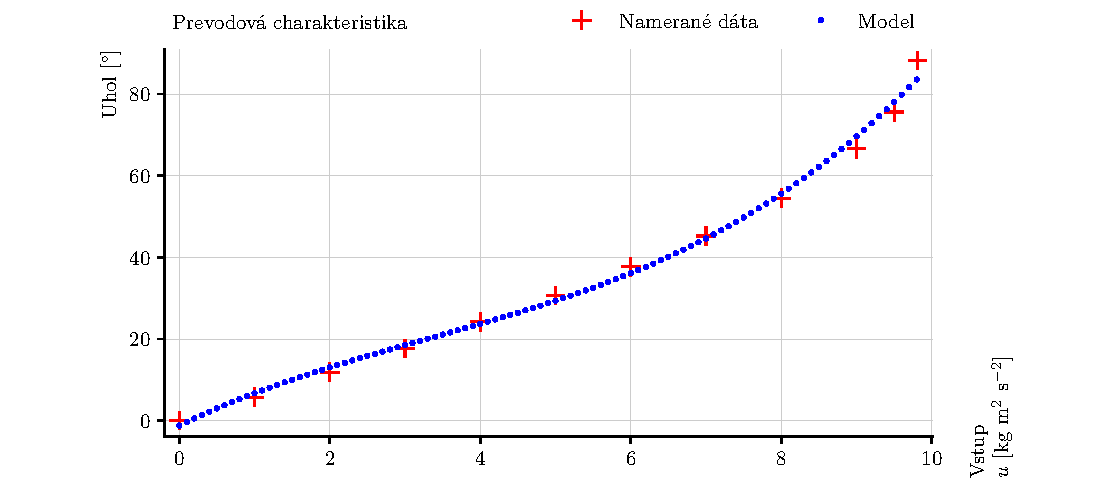
\includegraphics{../fig/cv07_fig_2.pdf}
	}

    \vspace{-4mm}

	\caption{}
	\label{Prevodová charakteristika graf2}

\end{figure}




\begin{figure}[t]
	\centering

    \makebox[\textwidth][c]{%
	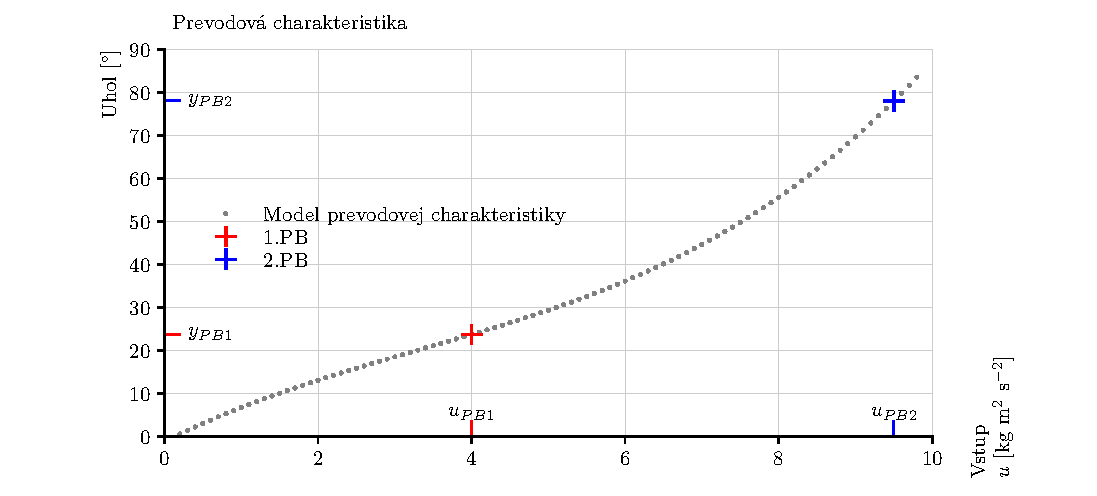
\includegraphics{../fig/cv07_fig_4.pdf}
	}

    \vspace{-4mm}

	\caption{}
	\label{Prevodová charakteristika graf4}

\end{figure}





\subsection{Stručné vysvetlenie pojmov}

Hlavnou úlohou v tomto texte je odmerať prechodové charakteristiky predmetného systému (laboratórny systém) v rôznych pracovných bodoch. Pracovné body nech sú zvolené s prihliadnutím na prevodovú charakteristiku systému. V prvom rade, čo je to \emph{pracovný bod}?


\bigskip


Pracovný bod je definovaný ustálenou hodnotou vstupného signálu, ku ktorej (jednoznačne) prislúcha ustálená hodnota výstupného signálu. Dvojica hodnôt, hodnota na vstupe a hodnota na výstupe, tvorí pracovný bod.

Ak je daná ustálená hodnota vstupného signálu, potom je možné pomocou prevodovej charakteristiky nájsť prislúchajúcu ustálenú hodnotu výstupného signálu.

Pojem pracovný bod na seba viaže aj pojem \emph{okolie pracovného bodu}. V okolí pracovného bodu sú vlastnosti systému relatívne rovnaké ako v pracovnom bode. Z hľadiska statických vlastností systému to znamená, že v okolí pracovného bodu sa sklon prevodovej charakteristiky relatívne nemení. Inými slovami, statické zosilnenie systému sa nemení. Rovnako aj dynamické vlastnosti systému sú v okolí pracovného bodu relatívne nemenné - časové konštanty systému sa nemenia.

V dvoch rôznych pracovných bodoch môže mať reálny systém napríklad rozdielne statické zosilnenie, teda statické vlastnosti. Statické zosilnenie systému v pracovnom bode je možné určiť na základe prevodovej charakteristiky. Je dané sklonom prevodovej charakteristiky v okolí pracovného bodu.

Prípadný rozdiel v statických vlastnostiach v rôznych pracovných bodoch však nehovorí nič o prípadnom rozdiele dynamických vlastnostiach systému. Dynamické vlastnosti je možné vyhodnocovať na základe prechodovej charakteristiky.

\emph{Prechodová charakteristika} je odozva systému na jednotkový skok.

Pod pojmom \emph{jednotkový skok} sa rozumie skoková zmena signálu (vstupného) a veľkosť tejto zmeny je jednotková. Je jednotková zmysle, že akúkoľvek veľkosť skokovej zmeny má zmysel (prípadne) vyjadriť ako násobok jednotkovej skokovej zmeny. Prirodzene sa predpokladá, že jednotková zmena je taká, že nespôsobí, že systém sa dostane mimo okolia pracovného bodu.







\section{O meraní prechodovej charakteristiky}


Pracovné body nech sú zvolené s prihliadnutím na prevodovú charakteristiku systému. Ako teda prihliadnuť? Ako už bolo uvedené, z prevodovej charakteristiky je zrejmé, že istá vlastnosť systému je iná pri nízkych hodnotách vstupného signálu a iná pri vysokých hodnotách. Tou vlastnosťou je statické zosilnenie. Iné než tzv. statické vlastnosti systému z prevodovej charakteristiky nie je možné vyčítať. Otázkou teda je či sú aj iné vlastnosti systému rozdielne pri rôznych hodnotách vstupného signálu.

\subsection{Voľba pracovných bodov}


Zvoľme preto dva pracovné body - jeden nech reprezentuje nízku hodnotu vstupného signálu a druhý vysokú:

\begin{table}[!ht]
    \centering
	\catcode`\-=12

    \caption{Zvolené pracovné body}
    \label{Zvolené pracovné body}

    \begin{tabular}{ccc}
        \toprule
        PB & hodnota & jednotky \\
        \midrule
        1. & $4$ & [kg m$^2$ s$^{-2}$] \\
        2. & $9,5$ & [kg m$^2$ s$^{-2}$] \\
        \bottomrule
    \end{tabular}

\end{table}



Na základe nameraných bodov prevodovej charakteristiky by sme mohli k~zvoleným ustáleným vstupným hodnotám priradiť výstupné hodnoty:

\noindent
\begin{tabular}{@{}l l}
    1.PB: & $y=24,2$ [°] \\
    2.PB: & $y=75,5$ [°]
\end{tabular}


\bigskip

Pracujme však s aproximáciou prevodovej charakteristiky, teda s jej modelom. Model nám umožní získať aj také informácie, ktoré neboli reálne namerané.

Pre $u = 4$ [kg m$^2$ s$^{-2}$] podľa modelu prevodovej charakteristiky prislúcha hodnota ustáleného výstupu:
\begin{equation}
    \hat y_{PB1} = 0,1111\ u_{PB1}^3  -1,1150\ u_{PB1}^2 + 8,9102\ u_{PB1}  -1,1770
\end{equation}
kde ak $u_{PB1} = 4$ [kg m$^2$ s$^{-2}$], potom $\hat y_{PB1} = 23,73$ [°]. Podobne pre $u = 9,5$ [kg m$^2$ s$^{-2}$] podľa modelu prevodovej charakteristiky prislúcha hodnota ustáleného výstupu $\hat y_{PB2} = 78,06$ [°]. Znázornime pracovné body - viď obr.~\ref{Prevodová charakteristika graf4}.






Ďalej je, samozrejme, potrebné vhodne zvoliť okolie pracovného bodu (pre každý pracovný bod). V podstate je potrebné voliť pracovný bod a prislúchajúce okolie pracovného bodu naraz. Len tu sme to pre lepšiu názornosť oddelili.

Pripomeňme, že v okolí pracovného bodu sa očakáva, že vlastnosti systému sú relatívne nemenné. Na základe prevodovej charakteristiky možno posúdiť statické vlastnosti systému. Na základe toho, pre 1. pracovný bod (PB1) zvoľme okolie $u = 4 \pm 0,8$ [kg m$^2$ s$^{-2}$]. Pre PB2 zvoľme $u = 9,5 \pm 0,25$ [kg m$^2$ s$^{-2}$]. Znázornime pracovné body a ich okolia - viď obr.~\ref{Prevodová charakteristika graf5}. Na obrázku~\ref{Prevodová charakteristika graf5} sú tiež vyznačené hranice okolia pracovného bodu, napr. $u_{PB1_l}$ ako dolná hranica okolia pracovného bodu a~$u_{PB1_h}$ ako horná hranica. K tomu zodpovedajúce hodnoty výstupnej veličiny, hodnoty $y_{PB1_l}$ a~$y_{PB1_h}$ sú taktiež vyznačené. Obdobne aj pre druhý pracovný bod.





\begin{figure}[t]
	\centering

    \makebox[\textwidth][c]{%
	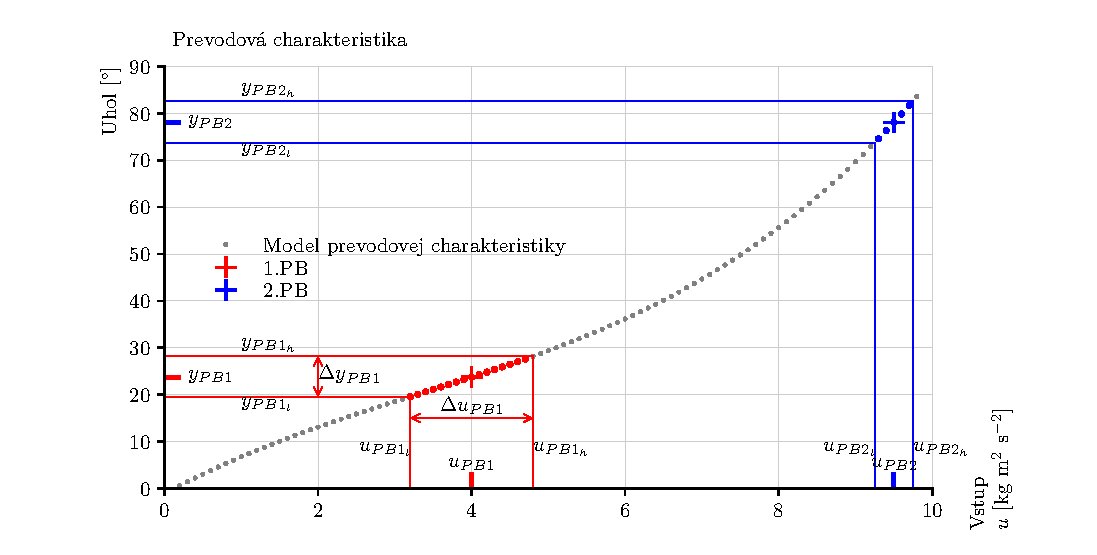
\includegraphics{../fig/cv07_fig_5.pdf}
	}

    \vspace{-4mm}

	\caption{}
	\label{Prevodová charakteristika graf5}

\end{figure}




Ďalej je v tomto prípade potrebné uvážiť veľkosť skokovej zmeny, ktorú budeme používať ako jednotkovú. Vzhľadom na okolnosti nie je dôvod, aby jednotkovou veľkosťou nebola hodnota definujúca okolie pracovného bodu. Spĺňa sa tak požiadavka, že jednotkový skok nespôsobí, že systém sa dostane mimo okolia pracovného bodu (bude na hrane, ale nie mimo). Preto pre PB1 nech je jednotková veľkosť skokovej zmeny rovná hodnote $u_{s1} = 0,8$ [kg m$^2$ s$^{-2}$] a pre PB2 nech je jednotková veľkosť skoku rovná hodnote $u_{s2} = 0,25$ [kg m$^2$ s$^{-2}$].






\subsection{Zrealizovanie merania prechodovej charakteristiky}


Aby bolo možné vykonať jednotkový skok (skokovú zmenu vstupného signálu systému s jednotkovou veľkosťou) v okolí pracovného bodu najskôr je potrebné dostať systém do pracovného bodu. Ak bude hodnota vstupného signálu $u_{PB}$, a necháme ju tak nejaký čas, potom očakávame, na základe prevodovej charakteristiky, že výstup systému sa ustáli na hodnote $y_{PB}$. Systém bude v pracovnom bode. Potom je možné skokovo zvýšiť hodnotu vstupného signálu o hodnotu $u_{s}$. Tým sa zrealizuje jednotkový skok v okolí pracovného bodu. Simulácia uvedeného je na obr.~\ref{graf6}.


\begin{figure}[t]
	\centering

    \makebox[\textwidth][c]{%
	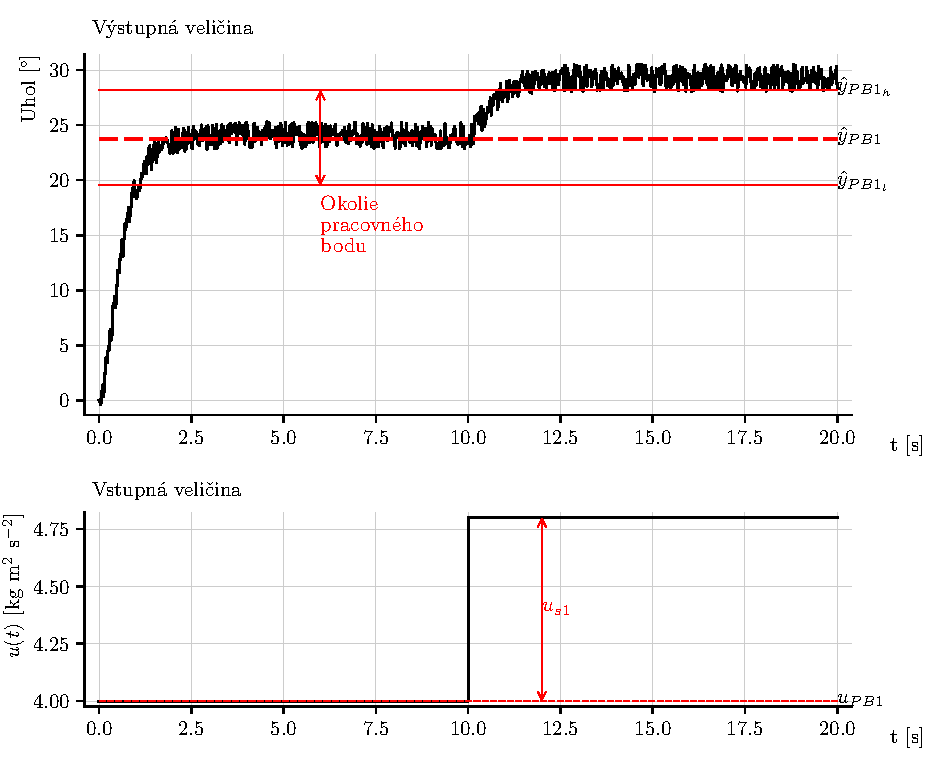
\includegraphics{../fig/cv07_fig_6.pdf}
	}

    \vspace{-4mm}

	\caption{}
	\label{graf6}

    \vspace{-4mm}

\end{figure}

Veľkosť skokovej zmeny vstupného signálu je na obrázku~\ref{graf6} označená ako $u_{s1}$. V~tomto prípade, vzhľadom na zvolené okolie pracovného bodu, je $u_{s1} = 0,8$.

Jednotkový skok nastal v čase $t=10$ [s]. Pred týmto časom sa systém dostával do pracovného bodu. Od času $t=10$ [s] až pokým sa výstupná veličina systému opäť neustálila prebieha prechodový dej, to je prechodová charakteristika (keďže na vstupe bol jednotkový skok).





















\begin{figure}[t]
	\centering

    \makebox[\textwidth][c]{%
	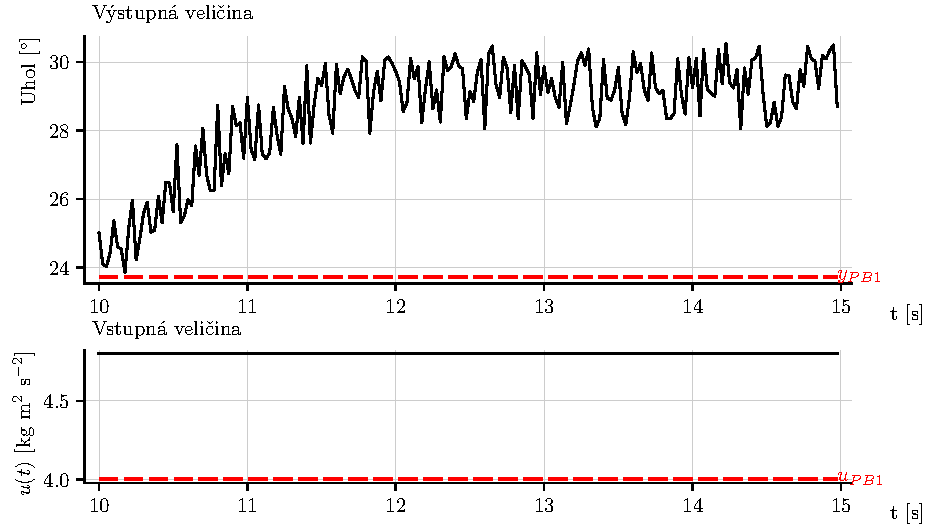
\includegraphics{../fig/cv07_fig_7.pdf}
	}

    \vspace{-4mm}

	\caption{}
	\label{graf7}

    \vspace{-4mm}

\end{figure}




\begin{figure}[!hb]
	\centering

    \makebox[\textwidth][c]{%
	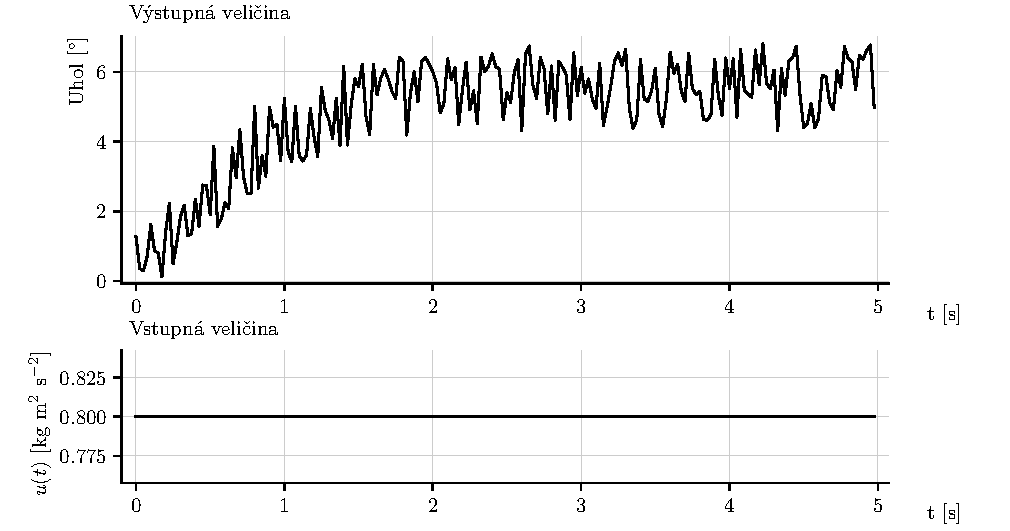
\includegraphics{../fig/cv07_fig_8.pdf}
	}

    \vspace{-4mm}

	\caption{}
	\label{graf8}

\end{figure}









\subsection{Spracovanie nameraného}


Pred jednotkovým skokom sme očakávali, že výstupná veličina sa ustáli na hodnote $y_{PB}$. Podľa modelu prevodovej charakteristiky to pre tento pracovný bod je hodnota $\hat y_{PB1} = 23,73$ [°]


Priemerná hodnota výstupnej veličiny počas doby 5 sekúnd pred jednotkovým skokom je $24,04$ [°]. Odchýlka priemernej hodnoty, okolo ktorej sa systém ustálil v~pracovnom bode, od očakávanej hodnoty podľa modelu prevodovej charakteristiky je približne 1 \%. To je samozrejme prijateľná odchýlka. Ďalej teda môžeme považovať hodnotu $\hat y_{PB1}$ podľa modelu prevodovej charakteristiky za hodnotu, na ktorej bola ustálená výstupná veličina pred skokovou zmenou vstupného signálu.

Po ukončení prechodového deja sa podľa modelu prevodovej charakteristiky očakáva, že výstupná veličina sa ustáli na hodnote $\hat y_{PB1_h} = 28,19$ [°]

Už z obr.~\ref{graf6} je zrejmé, že v skutočnosti sa výstupná veličina ustáli na o niečo vyššej hodnote. Presnejšie, ak uvažujeme časový úsek po jednotkovom skoku, na ktorom je už výstupná veličina ustálená, nech je to úsek 2,5 až 5 sekúnd po jednotkovom skoku, tak na tomto úseku je priemerná hodnota výstupnej veličiny $29,2$ [°].



Ak pri hodnote $y_{PB1}$ bol rozdiel medzi očakávaným (podľa modelu prevodovej charakteristiky) a nameraným priam zanedbateľný, pri hodnote $y_{PB1_h}$ to už nie je také jednoznačné. Nie je jednoznačné, že rozdiel je zanedbateľný. Tento problém však súvisí s meraním prevodovej charakteristiky a následnou voľbou modelu prevodovej charakteristiky, ktorý sme sa tu rozhodli používať pri odhadovaní očakávaných hodnôt $y_{PB1}$ a $y_{PB1_h}$. Ak sme sa raz rozhodli používať daný model prevodovej charakteristiky, potom s prípadnými odchýlkami, ktoré zjavne nie sú omyly, je potrebné počítať.

Týmto sme chceli povedať, že napriek tomu, že čo sa očakávaných hodnôt týka, po jednotkovom skoku výstupná veličina opustila očakávané okolie pracovného bodu. Avšak je to len očakávané, odhadované okolie (na základe modelu prevodovej charakteristiky). Odchýlky od „reálnych“ hodnôt sú prijateľné a teda môžeme pokračovať bez nutnosti prehodnotiť voľbu okolia pracovného bodu.








\subsubsection{„Vystrihnutie“ prechodovej charakteristiky}

Vyberme z dát na obr.~\ref{graf6} len tú časť, ktorá zodpovedá prechodovej charakteristike, teda dáta od času 10 až po ustálenie (nech je to čas 15). Výsledkom je obr.~\ref{graf7}.





\subsubsection{„Posunutie“ prechodovej charakteristiky}



Pre potreby ďalšej práce s prechodovou charaketristikou je zvyčajne výhodné posunúť namerané dáta tak aby začiatok prechodovej charakteristiky bol v bode (0,0), to znameá, že PCH začína v  čase 0 a hodnota výstupnej veličiny v začiatku je tiež nula (aspoň filozoficky).


Konkrétne: od získaného priebehu výstupnej veličiny je potrebné odčítať hodnotu $y_{PB}$, pretože tak sa začiatok posunie v smere osi y do nuly (filozoficky... teraz nám to asi bude kaziť šum). Rovnako priebeh vstupnej veličiny je potrebné posunúť v~smere osi o hodnotu $u_{PB}$. Samozrejme, od časového vektora je potrebné odčítať čas, v~ktorom nastal jednotkový skok. Výsledok je na obr.~\ref{graf8}.










\section{Poznámky k odčítavaniu hodnôt z grafu prechodovej charakteristiky}



\subsection{Nameraná prechodová charakteristika}

Z predchádzajúceho je dostupná nameraná a spracovaná prechodová charakteristika (PCH) predmetného systému. Ide o prechodovú charakteristiku v prvom pracovnom bode. Je zobrazená na obr.~\ref{graf8}.


% \begin{figure}[!b]
% 	\centering
%
%     \makebox[\textwidth][c]{%
% 	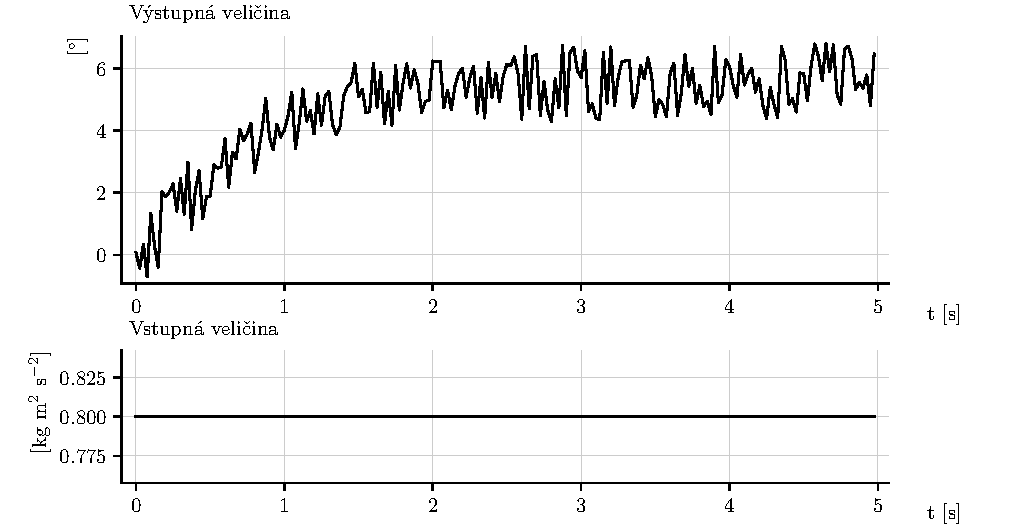
\includegraphics{../fig/cv08_fig_1.pdf}
% 	}
%
%     \vspace{-4mm}
%
% 	\caption{}
% 	\label{graf11}
%
% \end{figure}


Ďalej sú dostupné informácie o pracovnom bode, v ktorom bola PCH meraná. Hodnota vstupného signálu v pracovnom bode je $u = 4$ [kg m$^2$ s$^{-2}$] a uvažuje sa okolie pracovného bodu $u = 4 \pm 0,8$ [kg m$^2$ s$^{-2}$].

Je dostupný podel prevodovej charakteristiky a teda je možné odhadnúť hodnotu výstupnej veličiny v pracovnom bode, teda
\begin{equation}
    \hat y_{PB1} = 0,1111\ u_{PB1}^3  -1,1150\ u_{PB1}^2 + 8,9102\ u_{PB1}  -1,1770
\end{equation}
kde $u_{PB1} = 4$ [kg m$^2$ s$^{-2}$] a teda $\hat y_{PB1} = 23,73$ [°]. Rovnako je možné vypočítať hodnotu výstupného signálu pre, nazvime to, hornú hranicu okolia pracovného bodu, to znamená pre hodnotu na vstupe $u_{PB1_h} = 4 + 0,8$ [kg m$^2$ s$^{-2}$]. Tejto zodpovedá hodnota $\hat y_{PB1_h} = 28.19$ [°].

Keďže prechodová charakteristika na obr.~\ref{graf8} je posunutá do nuly, teda od skutočných hodnôt sú odčítané hodnoty v pracovnom bode, tak urobme túto úpravu aj pre práve vypočítané hodnoty, teda
\begin{align}
    \Delta u_{PB1} &= u_{PB1_h} - u_{PB1} = 0,8 \\
    \Delta \hat y_{PB1} &= \hat y_{PB1_h} -  \hat y_{PB1} = 4,52
\end{align}




\subsection{Statické zosilnenie $K$}

Zistime statické zosilnenie systému v okolí uvažovaného pracovného bodu. Potrebujeme hodnotu, na ktorej sa ustálila výstupná veličina po prechodovom deji. Z grafu PCH uvažujme, že výstupná veličina je už ustálená po čase $t=3$ [s] (dajme tomu teraz takto). Priemerná hodnota výstupnej veličiny po tomto čase je $\Delta y = 5.52$ [°].

Teda, po uskutočnení jednotkového skoku v okolí pracovného bodu sa výstupná veličina zmenila o $\Delta y$ [°]. Zmena na vstupe $\Delta u$ bola, samozrejme, práve jednotková (pretože jednotkový skok). V tomto prípade má jednotkový skok veľkosť okolia pracovného bodu  $\Delta u = 0,8$ [kg m$^2$ s$^{-2}$].

Statické zosilnenie systému, na základe prechodovej charakteristiky, označme $K$, je $K = \frac{\Delta y}{\Delta u}$, číselne
\begin{equation}
     K = 6,9 \text{[°/(kg m$^2$ s$^{-2}$)]}
\end{equation}
Uvedené možno znázorniť aj do grafu - viď obr.~\ref{graf20}


\begin{figure}[t]
	\centering

    \makebox[\textwidth][c]{%
	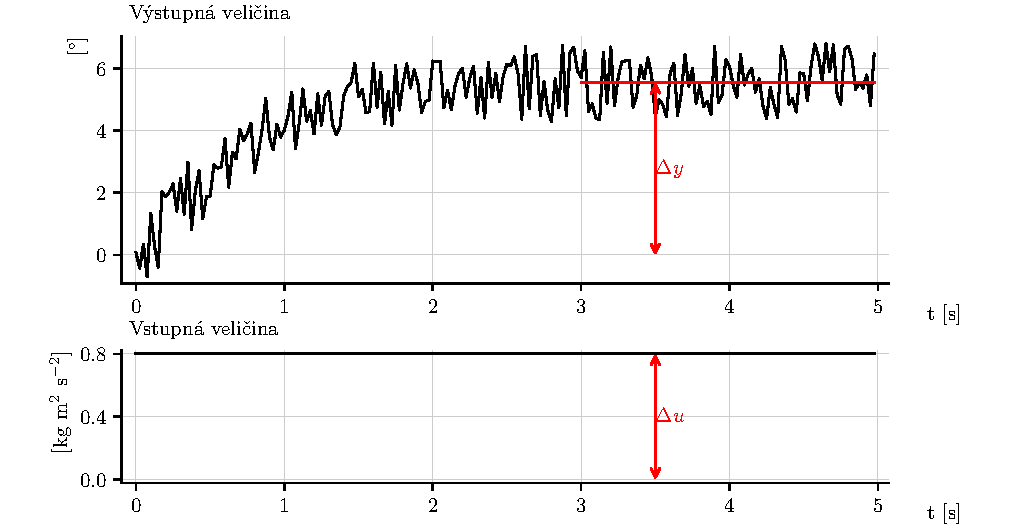
\includegraphics{../fig/cv08_fig_2.pdf}
	}

    \vspace{-4mm}

	\caption{}
	\label{graf20}

\end{figure}




Statické zosilnenie systému je, samozrejme, možné zistiť aj pomocou prevodovej charakteristiky. V skutočnosti, všetko potrebné už máme k dispozícii.

Mimochodom, ak by sme neboli leniví, tak nájdeme dotyčnicu v pracovnom bode, a jej smernica (sklon) by mala byť statické zosilnenie. To by bol formálne korektný postup.

My však leniví sme, preto: hľadáme sklon prevodovej charakteristiky v okolí pracovného bodu. Z praktického hľadiska, nech je sklon daný pracovným bodom a bodom ohraničujúcim okolie pracovného bodu zhora. Formálne $\text{sklon} = \frac{\Delta y}{\Delta u}$ kde $\Delta y = \hat y_{PB_h} - \hat y_{PB}$ a~$\Delta u = u_{PB_h} - u_{PB}$. To je, samozrejme, to isté ako vyplynulo z~využitia prechodovej charakteristiky vyššie. Tu však číselné hodnoty nie sú odčítané z~prechodovej charakteristiky ale z~modelu prevodovej charakteristiky. Konkrétne čísla:
\begin{equation}
    \text{sklon} = \frac{\hat y_{PB_h} - \hat y_{PB}}{u_{PB_h} - u_{PB}} = \frac{4,52}{0,8} = 5.65
\end{equation}
Odchýlka od statického zosilnenia určeného z prechodovej charakteristiky je $-1,25$ [°], t.j. $18,10$ [\%] (tá je samozrejme daná aj tým, že používame model prevodovej charakteristiky, keďže konkrétne potrebné hodnoty v rámci nameranej prevodovej charakteristiky nie sú dostupné).





\subsection[Časová konštanta $T$ pre lineárny dynamický systém 1. rádu]{Časová konštanta $T$ pre lineárny dynamický systém 1. rádu}


Ďalej je možné nájsť model, ktorý má vystihovať dynamiku (dynamické vlastnosti) reálneho systému. Modelom nech je lineárny dynamický systém.

Kvalifikovaný odhad založený na grafickom znázornení predmetnej prechodovej charakteristiky vedie k možnosti, že modelom systému môže byť dynamický systém 1. rádu. Tento je možné zapísať v tvare prenosovej funkcie
\begin{equation}
    G(s) = \frac{y(s)}{u(s)} = \frac{K}{Ts+1}
\end{equation}
kde $K$ je možné interpretovať ako statické zosilnenie systému a $T$ je časová konštanta.

Časovú konštantu je možné nájsť na základe prechodovej charakteristiky. Je to čas od začiatku prechodovej charakteristiky (od času jednotkového skoku), v ktorom výstupná veličina dosiahla približne 63 \% zo svojej ustálenej hodnoty.

Prečo práve 63 \%? Odpoveď sa ponecháva na čitateľa.

100 \% z ustálenej hodnoty na nasledujúcom obrázku~\ref{graf30} je samozrejme hodnota $\Delta y$. Potom 63 \% je hodnota $\Delta y_{63} =  3,48$ [°]



\begin{figure}[t]
	\centering

    \makebox[\textwidth][c]{%
	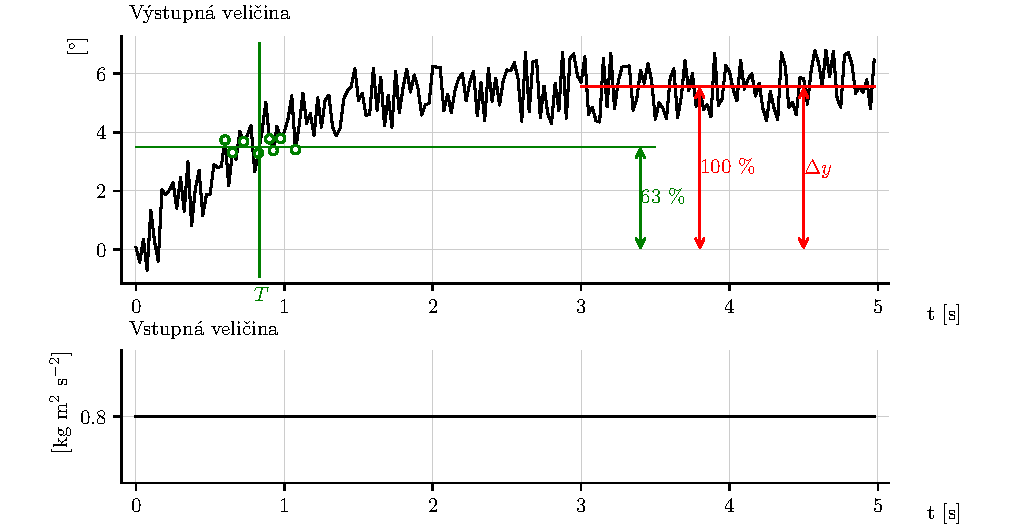
\includegraphics{../fig/cv08_fig_3.pdf}
	}

    \vspace{-4mm}

	\caption{}
	\label{graf30}

\end{figure}


Hodnotu $T$ teraz možno hľadať „od oka“, doslova pomocou grafu PCH, prípadne „od oka“, ale trošku inak - napr: Nájdime hodnoty výstupnej veličiny, ktoré sú v~pásme (volajme ho „od oka“) $\pm ? \%$ v okolí hodnoty $\Delta y_{63}$. Presnejšie, nájdime časy tých vzoriek, ktoré sú v~tom pásme. Nájdené body v~pásme „od oka“ okolo hodnoty $\Delta y_{63}$ sú na obr.~\ref{graf30} vyznačené ako malé zelené kružnice. Priemer z nájdených časov je
\begin{equation}
    T =  0,81 \text{[s]}
\end{equation}
A táto hodnota môže byť celkom dobre „od oka“ odčítaná časová konštanta. Všetko uvedené je nakreslené na obr.~\ref{graf30}.





\subsection{Verifikácia identifikovaného dynamického modelu}


V predchádzajúcom boli na základe prechodovej charakteristiky určené parametre lineárneho dynamického systému, ktorý má byť modelom skutočného systému. Tento model je možné vyjadriť v tvare prenosovej funkcie
\begin{equation}
    \frac{y(s)}{u(s)} = \frac{K}{Ts+1}
\end{equation}



Pre verifikáciu modelu je možné využiť grafické porovnanie prechodovej charakteristiky modelu a skutočnej prechodovej charakteristiky. Pre získanie PCH modelu využime numerickú simuláciu. Daná prenosová funkcia zodpovedá diferenciálnej rovnici v tvare
\begin{align}
    T \dot y(t) + y(t) &= K u(t) \\
    T \dot y(t) &= - y(t) + K u(t) \\
    \dot y(t) &= - \frac{1}{T} y(t) + \frac{K}{T} u(t)
\end{align}
Vstupný signál zvoľme rovnaký ako je veľkosť $\Delta u$. Tak zabezpečíme zodpovedajúcu veľkosť jednotkového skoku, ktorý je použitý v numerickej simulácii pre získanie PCH.

Do spoločného obrázka nakreslime nameranú PCH a PCH modelu systému - viď obr.~\ref{graf40}

\begin{figure}[t]
	\centering

    \makebox[\textwidth][c]{%
	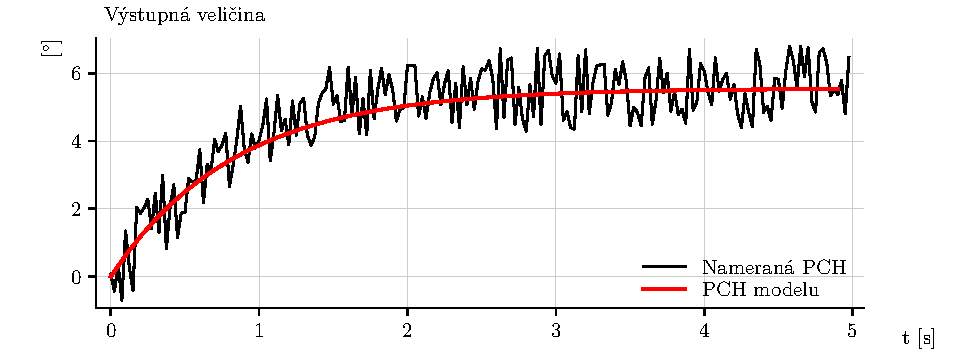
\includegraphics{../fig/cv08_fig_4.pdf}
	}

    \vspace{-4mm}

	\caption{}
	\label{graf40}

\end{figure}

Týmto (aspoň pre naše potreby) možno model považovať za verifikovaný - znamená to, že daný model je schopný vystihnúť vlastnosti skutočného systému a že je možné na základe dostupných informácií (prechodová charakteristika) nájsť parametre modelu.











\end{document}
